\documentclass{article}
\usepackage{amsmath, fullpage}
\usepackage{graphicx}
\begin{document}

\title{Nonlinear and Quantum Optics}
%\date{\vspace{-5ex}}
\maketitle
\thispagestyle{empty}
\tableofcontents

\section{Course outline}

The planned lectures are divided into four sections:
\begin{enumerate}
    \item Heuristic linear waves: classical, semi-classical, and quantum
    \item Nonlinear response: classical, semi-classical, and quantum
    \item Zoology of nonlinear effects: Pockels (DC Kerr), harmonic generation, stimulated four-wave-mixing, spontaneous four-wave mixing
    \item Silicon micro-ring resonator example: qualitative overview, experimental results, sketch of model (self-phase modulation, cross-phase modulation, two photon absorption, stimulated four-wave mixing, free carrier dispersion, free carrier absorption, thermo-optic effect)
\end{enumerate}

Some of the processes that we are trying to cover/understand are:

\begin{itemize}
    \item Squeezing
    \item Pair generation
    \item Self- and cross-phase modulation
    \item photon distinguishability
    \item discrete and continuous variable states
    \item ...
\end{itemize}

The course will not deal with detailed circuit-level applications. Rather, the emphasis is on developing fundamental and heuristic understanding of related physics.

\subsection{System definition}
For the systems to be studied in this course, we make the following assumptions:
\begin{enumerate}
    \item no magnetic effects
    \item no metal/plasmonics
    \item no active/resonance interactions
\end{enumerate}

\begin{figure}
    \label{fig:general_system}
    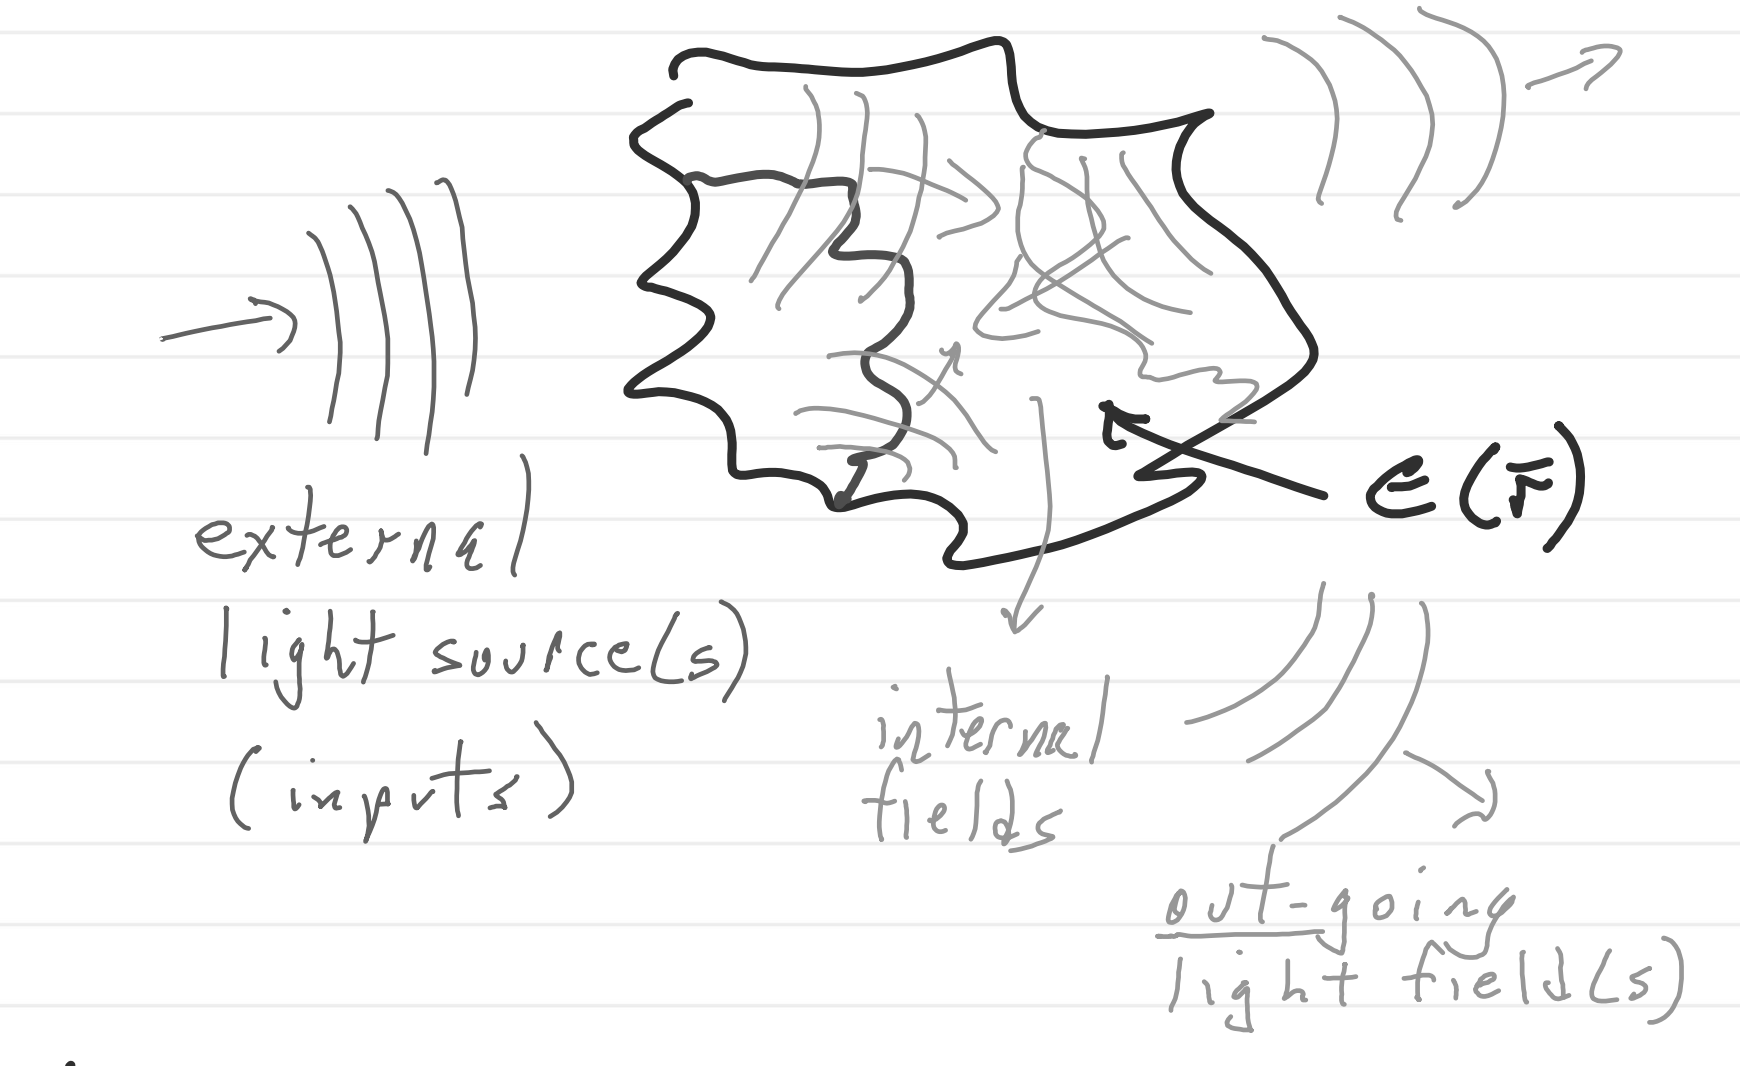
\includegraphics[width=0.6\textwidth]{figures/general_system_sketch.png}
    \centering
    \caption{h}
\end{figure}

We are fundamentally concerned with a nonlinear scattering problem, as illustrated in Figure \ref{fig:general_system}: There is an input electromagnetic field, which interacts with a dielectric environment characterized by $\epsilon(\vec{r})$, and emits out-going electromagnetic fields.

\subsection{Historical sidebar}
Nonlinear optics was historically investigated by irradiating a macroscopic nonlinear crystal with a powerful pulsed laser (Figure \ref{fig:nonlinear_crystal}). The laser is quasi-monochromatic with an angular frequency $\omega_0$, and the incoming field is 
\begin{equation}
    \vec{E}_{\rm{inc}} \sim \vec{E}_\alpha e^{i\left(\frac{\omega_0}{c}-\omega_0 t\right)},
\end{equation} 
where $\vec{E}_\alpha$ is the transverse field profile, $c$ is the speed of light, $z$ is position in the propagation direction, and $t$ is time. The crystal would emit very weak harmonics at $2\omega_0$, $3\omega_0$, and so on. The weak amplitudes of these harmonics was indicative of low conversion efficiency. 

Qualitatively, the generation of these harmonics can be understood as follows. Light is fundamentally an oscillating electromagnetic field. In a medium, this field will locally displace the charges via the Coulomb interaction. To lowest order, we can say that only the electrons are displaced, and the nuclei are stationary. A helpful analogy is to consider the electron-nucleus system to be a mass on a spring, where the spring constant is determined by the Coulomb interaction between the electron and the nucleus. At relatively low intensities, the angular frequency of the electron oscillation will be equal to that of the electromagnetic wave: $\omega_0 = \omega_{\rm{oscillation}}$. This is the linear regime. However, at high intensities, different frequency components can be excited.

\begin{figure}
    \label{fig:nonlinear_crystal}
    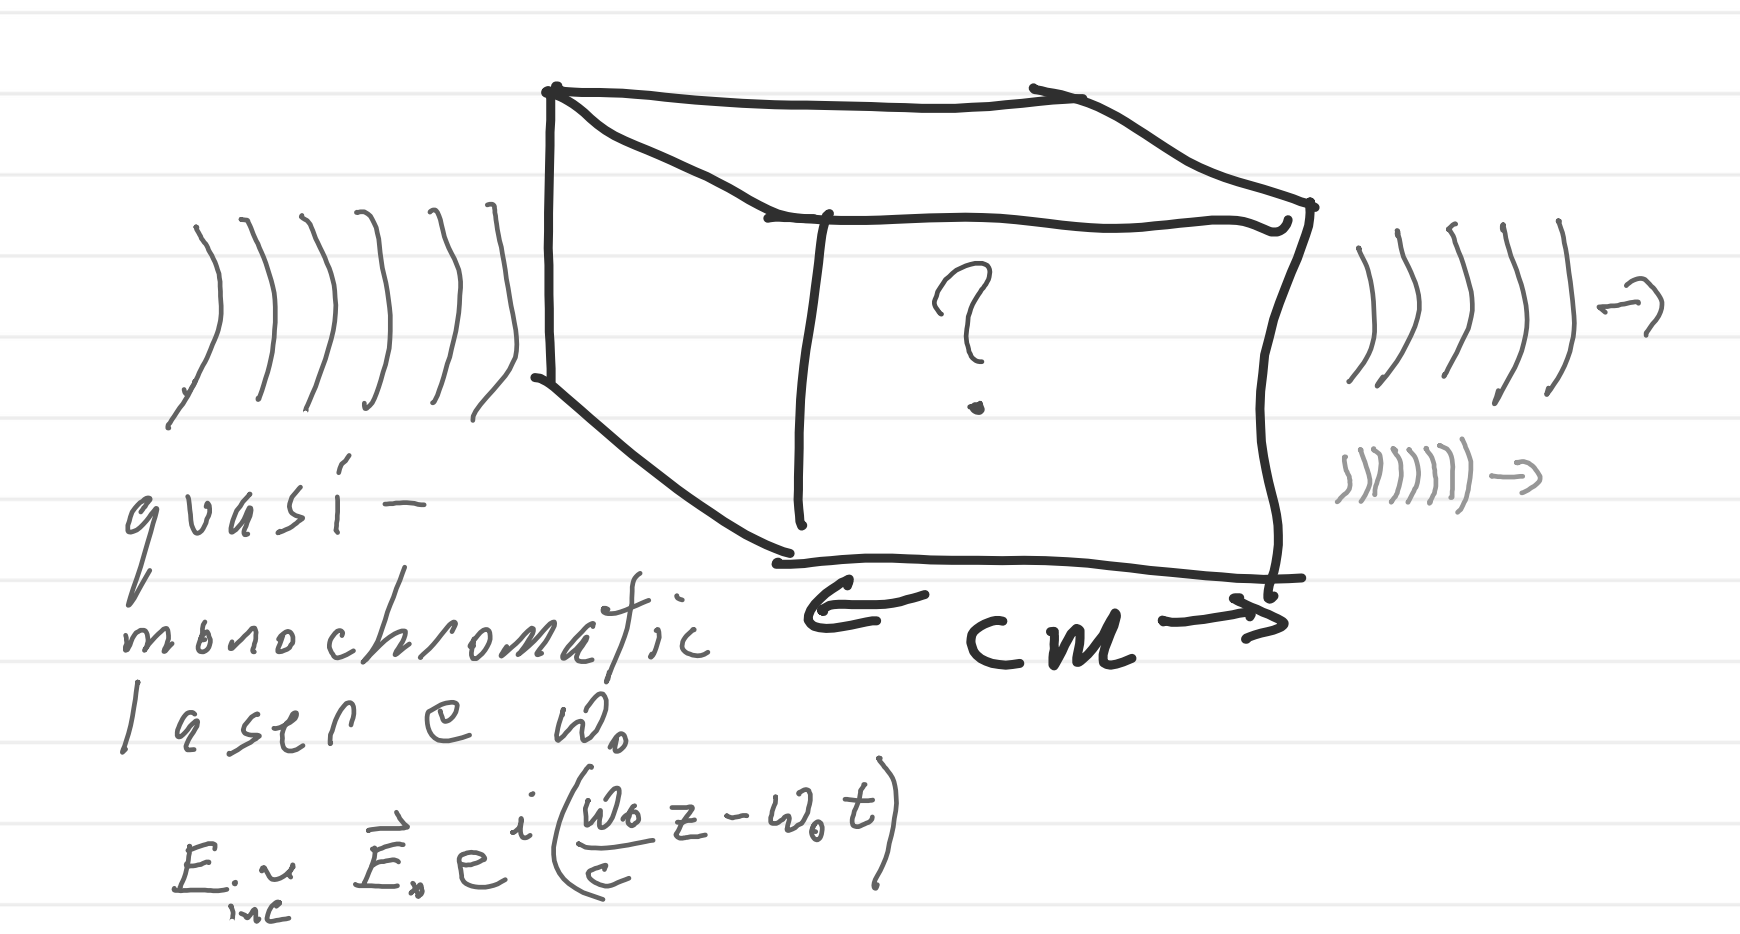
\includegraphics[width=0.6\textwidth]{figures/nonlinear_crystal.png}
    \centering
    \caption{h}
\end{figure}

\section{Heuristic linear propagation}
We will first begin with the simplest possible case of an incident wave normally-incident on a semi-infinite medium, as illustrated in Figure \ref{fig:plane_wave_normal_incidence}. The dielectric environment is invariant in the two transverse directions, and is divided into region I and region II at $z=0$. Let us assume that the incident field is a plane wave with angular frequency $\omega_{\rm{inc}}$ and free-space wavelength $\lambda_{\rm{inc}}$, and it is traveling in vacuum ($\epsilon=1$) in the positive z direction. We consider that the incident field is generated by a source that is external to our system. 

\begin{figure}
    \label{fig:plane_wave_normal_incidence}
    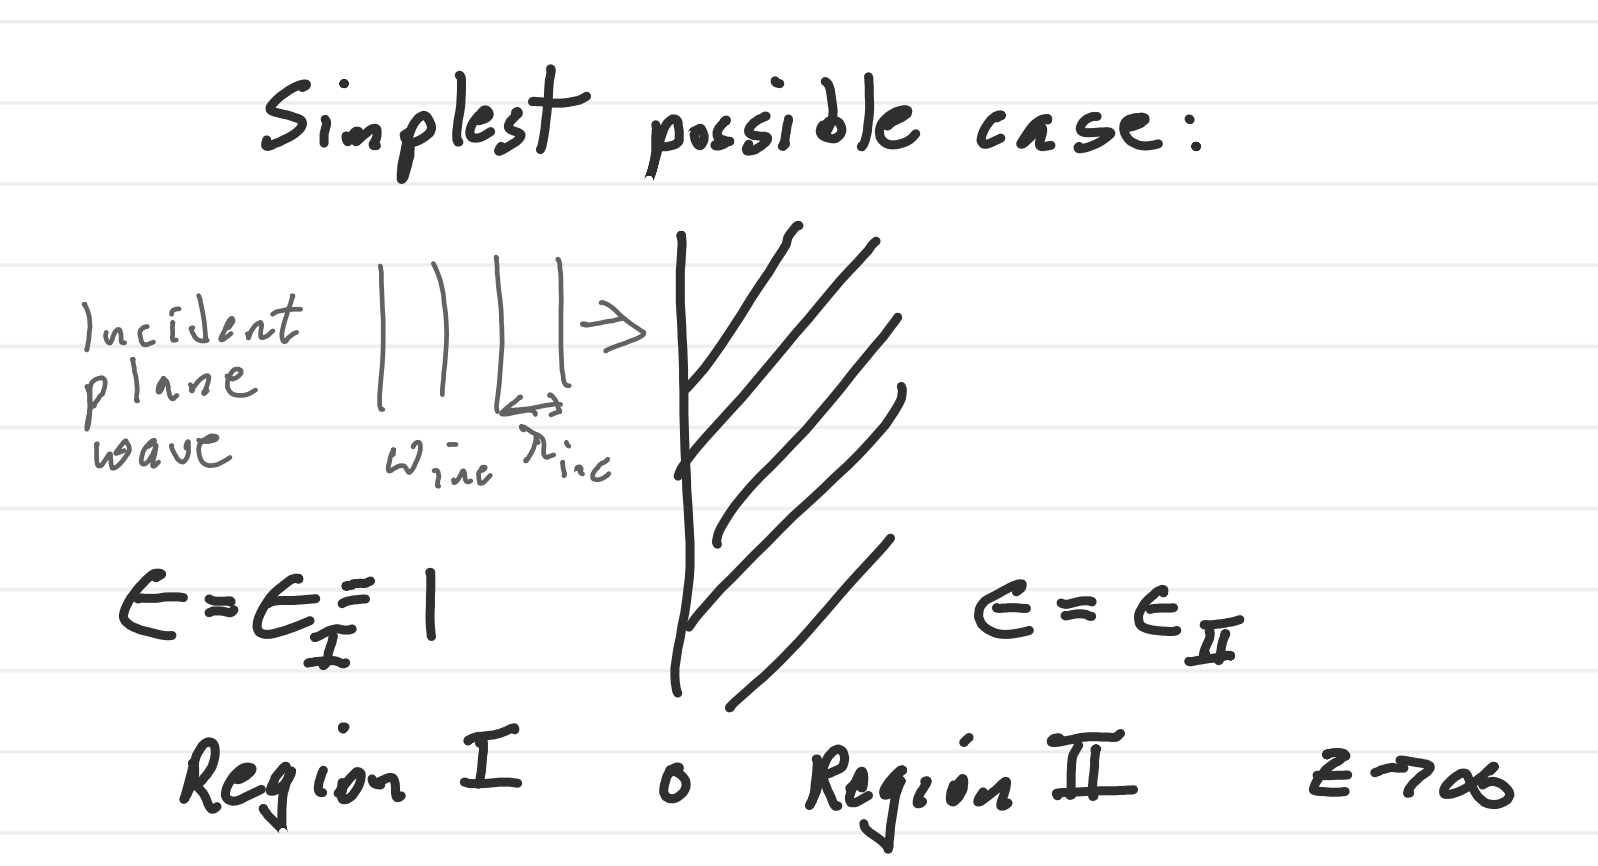
\includegraphics[width=0.6\textwidth]{figures/plane_wave_normal_incidence.png}
    \centering
    \caption{h}
\end{figure}

The main questions that we are concerned with are:
\begin{enumerate}
    \item What are the scattered fields?
    \item What is the source of the scattered fields?
\end{enumerate}

Immediately, we can give qualitative answers to these questions: There are two scattered fields: the transmitted field, and the reflected field. The source of these scattered fields is the oscillations of the electrons inside region II. We 

\subsection{Maxwell equations}
The fundamental, microscopic Maxwell equations written in cgs units are 
\begin{eqnarray}
    c\vec\nabla\times\vec e &= &-\dot{\vec{b}} \\
    c\vec\nabla\times\vec b &= &\dot{\vec{e}} + 4\pi \vec{J}_\mu \\
    \vec\nabla\cdot\vec b &= &0 \\
    \vec\nabla\cdot\vec e &= &4\pi \rho_\mu.
\end{eqnarray}

In mks units, they are
\begin{eqnarray}
    \vec\nabla\times\vec e &= &-\dot{\vec{b}} \\
    \vec\nabla\times\vec b &= &\epsilon_0 \mu_0 \dot{\vec{e}} + \mu_0\vec{J}_\mu \\
    \vec\nabla\cdot\vec b &= &0 \\
    \epsilon_0 \vec\nabla\cdot\vec e &= &\rho_\mu.
\end{eqnarray}

Here, $\vec e$ is the microscopic electric field, $\vec b$ is the microscopic magnetic field, $c$ is the speed of light, $\epsilon_0$ is the permittivity of free space, and $\mu_0$ is the permeability of free space. $\rho_\mu$ and $\vec{J}_\mu$ are the microscopic charge density and current density, respectively, and are given in general by 
\begin{eqnarray}
    \rho_\mu = \sum_{i}^{} q_i \delta(\vec r - \vec r_i(t)) \\
    \vec{J}_\mu = \sum_{i}^{} q_i \vec{v}_i \delta(\vec r - \vec r_i(t)),
\end{eqnarray}
where the sums are over discrete charge carriers $i$ at time-dependent positions $\vec{r}_i(t)$, with drift velocities $\vec v_i$. We assume the charges are classical here. The charges in a crystal are represented in Figure \ref{fig:crystal_cartoon}.

\begin{figure}
    \label{fig:crystal_cartoon}
    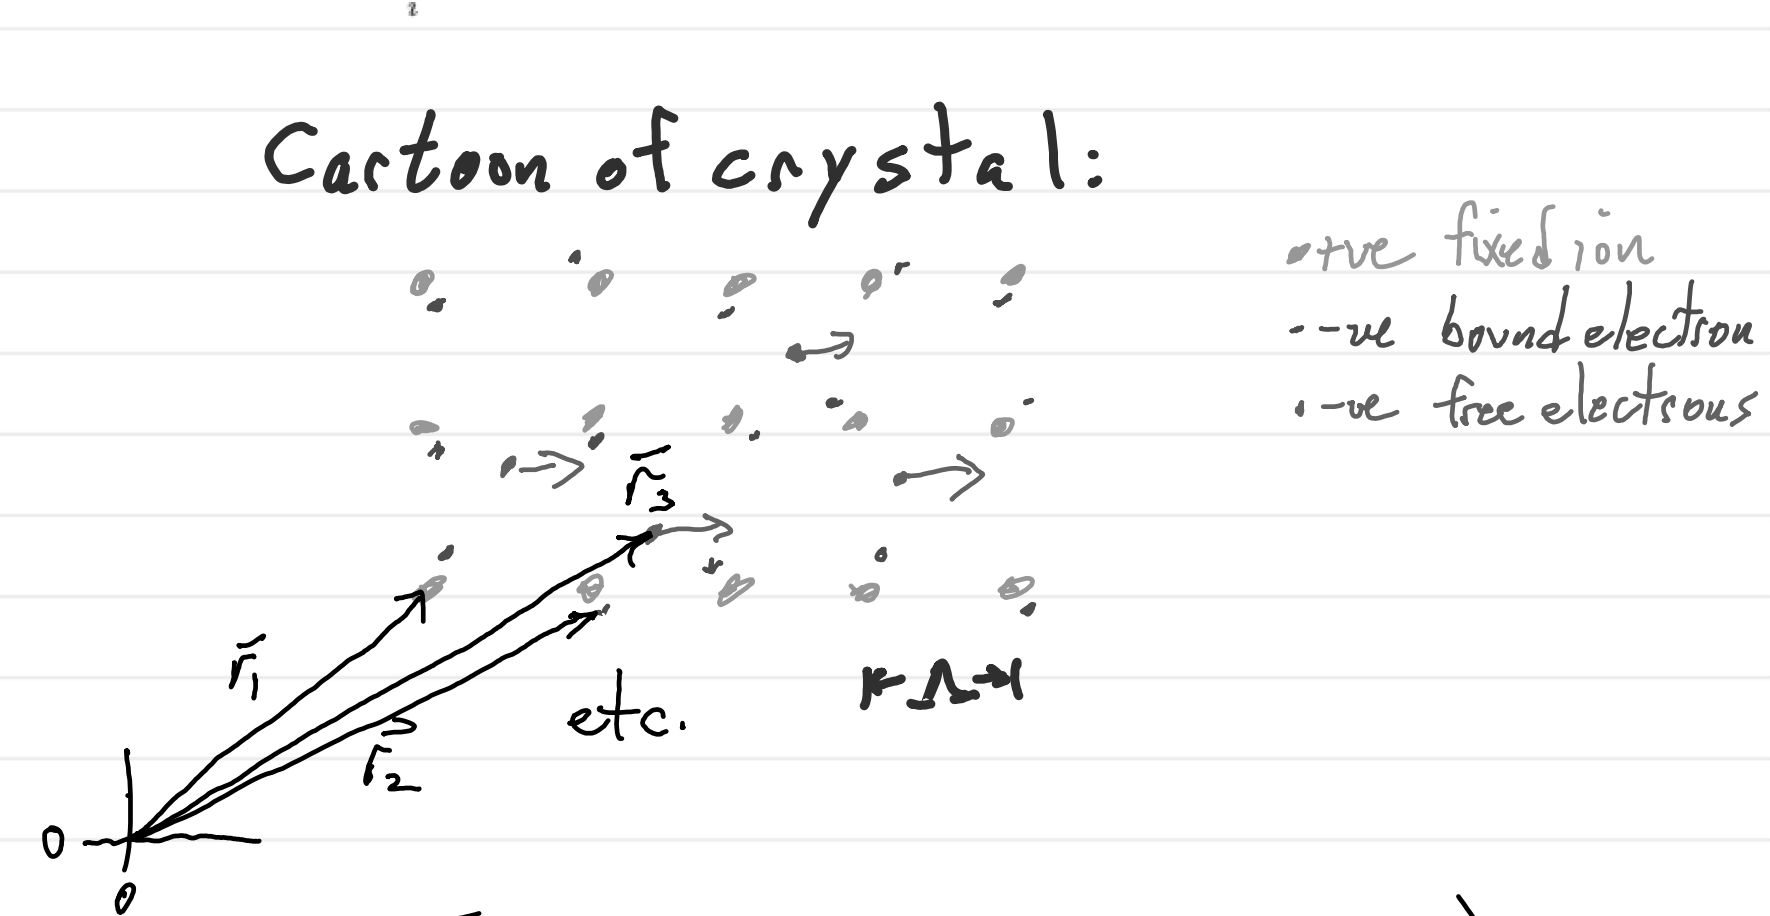
\includegraphics[width=0.6\textwidth]{figures/crystal_cartoon.png}
    \centering
    \caption{h}
\end{figure}

The microscopic Maxwell equations are exact: given $\rho_\mu$ and $\vec{J}_\mu$, we can solve these equations and obtain an exact solution for the fields. More practically, however, there is a need to make approximations. Typically, we average all physical quantities over a volume of some radius $R$, where the radius is much smaller than the wavelength in the medium ($R\ll\lambda$), but much larger than the atomic spacing ($R\gg\Lambda$).


The Maxwell equations tell us that the charges produce $\vec e$ and $\vec b$. However, they do not tell us how $\vec e$ and $\vec b$ act upon the charges. To solve for the dynamics of a given charge distribution, we need the Lorentz equation, which reads
\begin{equation}
    m_i \ddot{\vec{r}}_i = q_i \vec e(\vec{r}_i) + \dot{\vec{r}}_i\times\vec b(\vec{r}_i),
\end{equation}
where $m_i$ is the mass of charge $i$. The Lorentz equation tells us that fields locally exert forces on charges.


\end{document}
